\documentclass{beamer}
\usetheme{Madrid}
\usecolortheme{default}

\usepackage{amsmath}
\usepackage{algorithm}
\usepackage{algorithmic}
\usepackage{graphicx}
\usepackage{booktabs}
\usepackage{adjustbox}
\usepackage{makecell}
\usepackage{colortbl}
\usepackage{tikz}
\usepackage{pgfplots}
\pgfplotsset{compat=1.18}
\usetikzlibrary{shapes.geometric, arrows.meta, positioning, calc, patterns, decorations.pathreplacing, fit, backgrounds}

% Custom colors for visual consistency
\definecolor{cropgreen}{RGB}{76, 175, 80}
\definecolor{cropgold}{RGB}{255, 193, 7}
\definecolor{croporange}{RGB}{255, 152, 0}
\definecolor{cropblue}{RGB}{33, 150, 243}
\definecolor{croppurple}{RGB}{156, 39, 176}
\definecolor{synergyglow}{RGB}{255, 235, 59}
\definecolor{benefitgreen}{RGB}{129, 199, 132}
\definecolor{penaltyred}{RGB}{239, 154, 154}

\title{Building a Realistic Food Production Model}
\subtitle{Modular Enhancements for Agricultural Optimization}
\author{Edoardo Spigarolo}
\date{\today}

\begin{document}

\frame{\titlepage}

\begin{frame}{The Challenge}

\textbf{We have a working optimization model for food production.}

\vspace{0.5cm}

But real agriculture is more complex than our simple model assumes:

\vspace{0.3cm}

\begin{itemize}
    \item[\textcolor{cropgreen}{\textbullet}] \textbf{Markets don't scale linearly} --- growing twice as much wheat doesn't mean twice the profit
    
    \vspace{0.2cm}
    
    \item[\textcolor{cropgold}{\textbullet}] \textbf{Crops interact with each other} --- some plants help their neighbors grow better
    
    \vspace{0.2cm}
    
    \item[\textcolor{croppurple}{\textbullet}] \textbf{What you planted last year matters} --- soil health depends on crop sequences
\end{itemize}

\vspace{0.5cm}

\textbf{Question:} How do we add these real-world effects to our model?

\end{frame}

\begin{frame}{What We'll Explore Together}

\textbf{Three ways to make our model more realistic:}

\vspace{0.5cm}

\begin{enumerate}
    \item \textcolor{cropgreen}{\textbf{Diminishing Returns}}\\
    \textit{``The more you grow of one crop, the less valuable each additional hectare becomes''}\\
    \scriptsize Think: market saturation, labor limits, pest buildup
    
    \vspace{0.4cm}
    
    \item \normalsize\textcolor{cropgold}{\textbf{Companion Planting (Synergy)}}\\
    \textit{``Some crops grow better when planted near each other''}\\
    \scriptsize Think: nitrogen-fixing legumes helping cereals, pest deterrence
    
    \vspace{0.4cm}
    
    \item \normalsize\textcolor{croppurple}{\textbf{Crop Rotation}}\\
    \textit{``Planning what to plant this year based on what grew last year''}\\
    \scriptsize Think: soil recovery, disease cycle breaking, nutrient replenishment
\end{enumerate}

\vspace{0.4cm}

\textbf{Your expertise helps us decide:} Which effects matter most for your crops?

\end{frame}

\begin{frame}{A Modular Optimization Approach}

\begin{center}
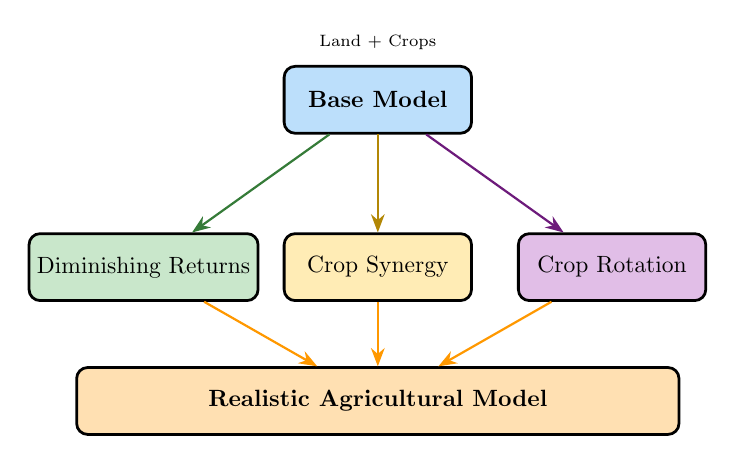
\begin{tikzpicture}[scale=0.85, transform shape,
    block/.style={rectangle, rounded corners, minimum width=2.8cm, minimum height=1cm, text centered, draw=black, line width=1pt},
    arrow/.style={-Stealth, thick}
]
% Base model
\node[block, fill=cropblue!30] (base) at (0,0) {\textbf{Base Model}};
\node[above=0.1cm of base, font=\scriptsize] {Land + Crops};

% Enhancement blocks
\node[block, fill=cropgreen!30] (dim) at (-3.5,-2.5) {Diminishing Returns};
\node[block, fill=cropgold!30] (syn) at (0,-2.5) {Crop Synergy};
\node[block, fill=croppurple!30] (rot) at (3.5,-2.5) {Crop Rotation};

% Arrows
\draw[arrow, cropgreen!70!black] (base) -- (dim);
\draw[arrow, cropgold!70!black] (base) -- (syn);
\draw[arrow, croppurple!70!black] (base) -- (rot);

% Plus signs
% \node at (-1.75,-1.25) {\Large\textcolor{gray}{+}};
% \node at (0,-1.25) {\Large\textcolor{gray}{+}};
% \node at (1.75,-1.25) {\Large\textcolor{gray}{+}};

% Output
\node[block, fill=croporange!30, minimum width=9cm] (real) at (0,-4.5) {\textbf{Realistic Agricultural Model}};
\draw[arrow, thick, croporange] (dim) -- (real);
\draw[arrow, thick, croporange] (syn) -- (real);
\draw[arrow, thick, croporange] (rot) -- (real);
\end{tikzpicture}
\end{center}



\end{frame}

% \begin{frame}{Problem Overview}
% \frametitle{What We're Optimizing}

% \begin{columns}
% \begin{column}{0.55\textwidth}
% \textbf{Goal:} Allocate land across farms to grow crops that maximize:
% \begin{itemize}
%     \item Nutritional value
%     \item Sustainability
%     \item Affordability
%     \item Environmental impact
% \end{itemize}

% \vspace{0.3cm}
% \textbf{Constraints:}
% \begin{itemize}
%     \item Available land per farm
%     \item Crop diversity requirements
%     \item Minimum viable plot sizes
% \end{itemize}
% \end{column}

% \begin{column}{0.45\textwidth}
% \begin{tikzpicture}[scale=0.7, transform shape]
% % Farm visualization
% \draw[thick, fill=cropgreen!20] (0,0) rectangle (4,3);
% \draw[thick, fill=cropgold!40] (0,0) rectangle (1.5,1.5);
% \draw[thick, fill=cropblue!40] (1.5,0) rectangle (4,1.5);
% \draw[thick, fill=croporange!40] (0,1.5) rectangle (2.5,3);
% \draw[thick, fill=croppurple!40] (2.5,1.5) rectangle (4,3);

% % Labels
% \node at (0.75,0.75) {\scriptsize Wheat};
% \node at (2.75,0.75) {\scriptsize Corn};
% \node at (1.25,2.25) {\scriptsize Legumes};
% \node at (3.25,2.25) {\scriptsize Veg};

% % Farm label
% \node[above] at (2,3.2) {\textbf{Farm Layout}};

% % Area notation
% \draw[<->, thick] (4.3,0) -- (4.3,3);
% \node[right] at (4.3,1.5) {\scriptsize $L_f$};
% \end{tikzpicture}
% \end{column}
% \end{columns}

% \end{frame}

\begin{frame}{The Base Model: Simple Linear Allocation}

\begin{columns}
\begin{column}{0.5\textwidth}
\textbf{Core Objective:}
\begin{equation*}
\max \sum_{\text{farms}} \sum_{\text{crops}} \underbrace{B_c}_{\text{benefit}} \times \underbrace{A_{f,c}}_{\text{area}}
\end{equation*}

\vspace{0.3cm}
\textbf{What $B_c$ captures:}
\begin{itemize}
    \item Nutritional score
    \item Sustainability index
    \item Affordability rating
    \item Environmental impact
\end{itemize}
\end{column}

\begin{column}{0.5\textwidth}
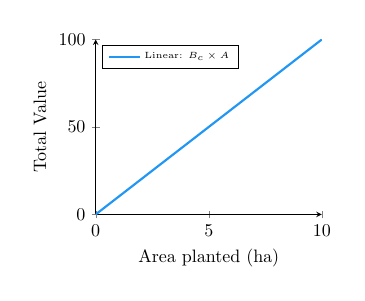
\begin{tikzpicture}[scale=0.65, transform shape]
% Linear value visualization
\begin{axis}[
    xlabel={Area planted (ha)},
    ylabel={Total Value},
    xmin=0, xmax=10,
    ymin=0, ymax=100,
    width=6cm, height=5cm,
    axis lines=left,
    xtick={0,5,10},
    ytick={0,50,100},
    legend pos=north west,
    legend style={font=\tiny}
]
\addplot[cropblue, very thick, domain=0:10] {10*x};
\addlegendentry{Linear: $B_c \times A$}
\end{axis}
\end{tikzpicture}

\vspace{0.2cm}
\centering
\scriptsize \textit{Value grows proportionally with area}
\end{column}
\end{columns}

\vspace{0.3cm}
\textbf{Limitation:} Assumes doubling the area always doubles the value

\end{frame}

\begin{frame}{Notation Quick Reference}

\begin{columns}
\begin{column}{0.5\textwidth}
\textbf{Sets \& Parameters}
\begin{itemize}
    \item $\mathcal{F}$: Set of farms
    \item $\mathcal{C}$: Set of crops  
    \item $\mathcal{G}$: Food groups
    \item $L_f$: Land available on farm $f$
    \item $B_c$: Composite value of crop $c$
\end{itemize}
\end{column}

\begin{column}{0.5\textwidth}
\textbf{Decision Variables}
\begin{itemize}
    \item $A_{f,c}$: Area for crop $c$ on farm $f$
    \item $Y_{f,c}$: Is crop $c$ planted on $f$? 
\end{itemize}

\vspace{0.3cm}
\textbf{Key Constraints}
\begin{itemize}
    \item $\sum_c A_{f,c} \leq L_f$ \scriptsize(land limit)
    \item \normalsize Diversity requirements (food groups)
\end{itemize}
\end{column}
\end{columns}

\end{frame}

\begin{frame}{Two Approaches: Continuous vs Binary}

\begin{center}
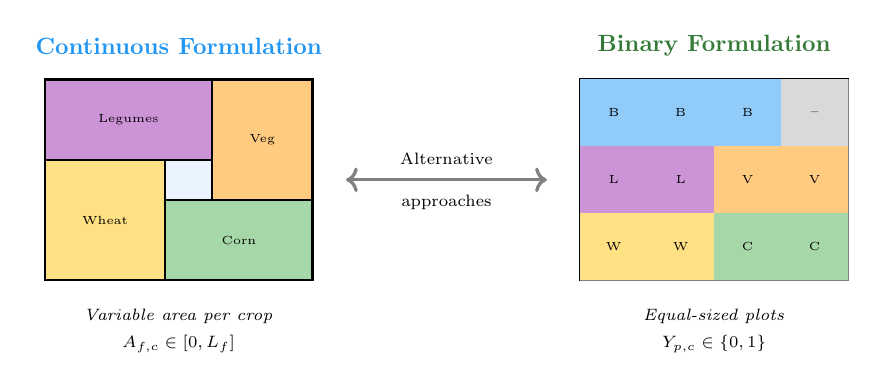
\begin{tikzpicture}[scale=0.85, transform shape]
% Left side - Continuous
\node[font=\bfseries, cropblue] at (-4,3.5) {Continuous Formulation};

% Farm with variable areas
\draw[thick, fill=cropblue!10] (-6,0) rectangle (-2,3);
\draw[thick, fill=cropgold!50] (-6,0) rectangle (-4.2,1.8);
\draw[thick, fill=cropgreen!50] (-4.2,0) rectangle (-2,1.2);
\draw[thick, fill=croppurple!50] (-6,1.8) rectangle (-3.5,3);
\draw[thick, fill=croporange!50] (-3.5,1.2) rectangle (-2,3);

\node[font=\tiny] at (-5.1,0.9) {Wheat};
\node[font=\tiny] at (-3.1,0.6) {Corn};
\node[font=\tiny] at (-4.75,2.4) {Legumes};
\node[font=\tiny] at (-2.75,2.1) {Veg};

\node[font=\scriptsize, below] at (-4,-0.3) {\textit{Variable area per crop}};
\node[font=\scriptsize, below] at (-4,-0.7) {$A_{f,c} \in [0, L_f]$};

% Right side - Binary
\node[font=\bfseries, cropgreen!70!black] at (4,3.5) {Binary Formulation};

% Even grid
\draw[thick, fill=cropgreen!10] (2,0) rectangle (6,3);
\foreach \x in {2,3,4,5} {
    \foreach \y in {0,1,2} {
        \draw[gray] (\x,\y) rectangle (\x+1,\y+1);
    }
}
% Fill some plots
\fill[cropgold!50] (2,0) rectangle (3,1);
\fill[cropgold!50] (3,0) rectangle (4,1);
\fill[cropgreen!50] (4,0) rectangle (5,1);
\fill[cropgreen!50] (5,0) rectangle (6,1);
\fill[croppurple!50] (2,1) rectangle (3,2);
\fill[croppurple!50] (3,1) rectangle (4,2);
\fill[croporange!50] (4,1) rectangle (5,2);
\fill[croporange!50] (5,1) rectangle (6,2);
\fill[cropblue!50] (2,2) rectangle (3,3);
\fill[cropblue!50] (3,2) rectangle (4,3);
\fill[cropblue!50] (4,2) rectangle (5,3);
\fill[gray!30] (5,2) rectangle (6,3);

\node[font=\tiny] at (2.5,0.5) {W};
\node[font=\tiny] at (3.5,0.5) {W};
\node[font=\tiny] at (4.5,0.5) {C};
\node[font=\tiny] at (5.5,0.5) {C};
\node[font=\tiny] at (2.5,1.5) {L};
\node[font=\tiny] at (3.5,1.5) {L};
\node[font=\tiny] at (4.5,1.5) {V};
\node[font=\tiny] at (5.5,1.5) {V};
\node[font=\tiny] at (2.5,2.5) {B};
\node[font=\tiny] at (3.5,2.5) {B};
\node[font=\tiny] at (4.5,2.5) {B};
\node[font=\tiny] at (5.5,2.5) {--};

\node[font=\scriptsize, below] at (4,-0.3) {\textit{Equal-sized plots}};
\node[font=\scriptsize, below] at (4,-0.7) {$Y_{p,c} \in \{0, 1\}$};

% Arrow between
\draw[<->, very thick, gray] (-1.5,1.5) -- (1.5,1.5);
\node[font=\scriptsize, above] at (0,1.6) {Alternative};
\node[font=\scriptsize, below] at (0,1.4) {approaches};
\end{tikzpicture}
\end{center}

\end{frame}

\begin{frame}{Why Binary? Quantum Hardware Compatibility}

\begin{columns}
\begin{column}{0.55\textwidth}
\textbf{Quantum computers work with binary:}
\begin{itemize}
    \item Qubits are naturally 0 or 1
    \item No continuous variables on quantum hardware
    \item Direct mapping to QUBO problems
\end{itemize}

\vspace{0.3cm}
\textbf{Binary formulation enables:}
\begin{itemize}
    \item \textcolor{cropgreen!70!black}{Pure quantum solving}
    \item \textcolor{cropgreen!70!black}{Hybrid quantum-classical}
    \item \textcolor{cropgreen!70!black}{Potential speedup for large problems}
\end{itemize}

\vspace{0.3cm}
\textbf{Trade-off:}\\
\scriptsize Less precision (discrete plots) but quantum-ready
\end{column}

\begin{column}{0.45\textwidth}
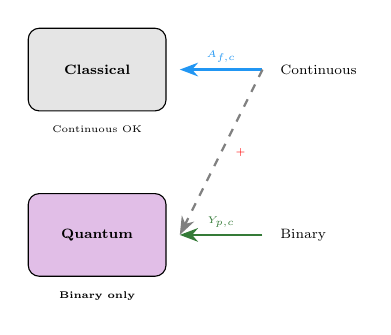
\begin{tikzpicture}[scale=0.7, transform shape]
% Classical computer
\node[rectangle, rounded corners, draw, fill=gray!20, minimum width=2.5cm, minimum height=1.5cm] (classical) at (0,3) {};
\node[font=\scriptsize\bfseries] at (0,3) {Classical};
\node[font=\tiny, below] at (0,2.1) {Continuous OK};

% Quantum computer
\node[rectangle, rounded corners, draw, fill=croppurple!30, minimum width=2.5cm, minimum height=1.5cm] (quantum) at (0,0) {};
\node[font=\scriptsize\bfseries] at (0,0) {Quantum};
\node[font=\tiny, below] at (0,-0.9) {\textbf{Binary only}};

% Arrows
\draw[-Stealth, thick, cropblue] (3,3) -- node[above, font=\tiny] {$A_{f,c}$} (1.5,3);
\draw[-Stealth, thick, cropgreen!70!black] (3,0) -- node[above, font=\tiny] {$Y_{p,c}$} (1.5,0);
\draw[-Stealth, thick, gray, dashed] (3,3) -- (1.5,0);
\node[font=\tiny, rotate=-45] at (2.6,1.5) {\textcolor{red}{$\times$}};

% Labels
\node[font=\scriptsize, right] at (3.2,3) {Continuous};
\node[font=\scriptsize, right] at (3.2,0) {Binary};
\end{tikzpicture}
\end{column}
\end{columns}

\end{frame}

\begin{frame}{Quantum Advantage: Binary vs Continuous}

\begin{center}
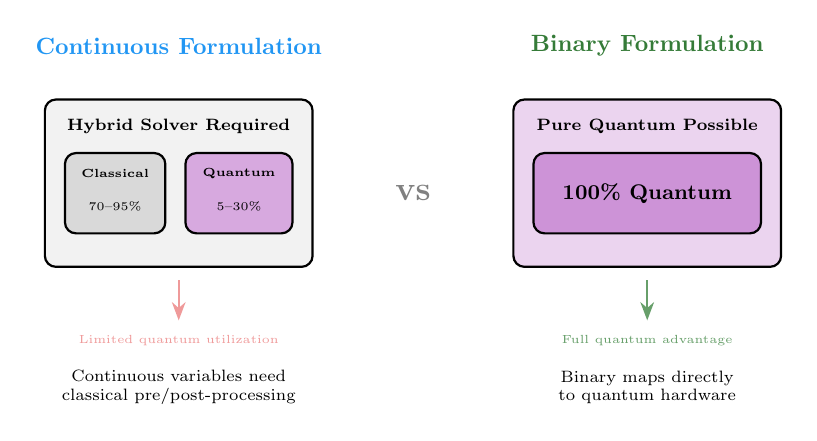
\begin{tikzpicture}[scale=0.85, transform shape]
% Left side - Continuous with Hybrid
\node[font=\bfseries, cropblue] at (-3.5,3.8) {Continuous Formulation};

% Hybrid solver box
\draw[thick, rounded corners, fill=gray!10] (-5.5,0.5) rectangle (-1.5,3);
\node[font=\scriptsize\bfseries] at (-3.5,2.6) {Hybrid Solver Required};

% Classical part
\draw[thick, fill=gray!30, rounded corners] (-5.2,1) rectangle (-3.7,2.2);
\node[font=\tiny\bfseries] at (-4.45,1.9) {Classical};
\node[font=\tiny] at (-4.45,1.4) {70--95\%};

% Quantum part (small)
\draw[thick, fill=croppurple!40, rounded corners] (-3.4,1) rectangle (-1.8,2.2);
\node[font=\tiny\bfseries] at (-2.6,1.9) {Quantum};
\node[font=\tiny] at (-2.6,1.4) {5--30\%};

% Arrow showing bottleneck
\draw[-Stealth, thick, penaltyred] (-3.5,0.3) -- (-3.5,-0.3);
\node[font=\tiny, penaltyred, below] at (-3.5,-0.4) {Limited quantum utilization};

% Right side - Binary with Pure Quantum
\node[font=\bfseries, cropgreen!70!black] at (3.5,3.8) {Binary Formulation};

% Pure quantum box
\draw[thick, rounded corners, fill=croppurple!20] (1.5,0.5) rectangle (5.5,3);
\node[font=\scriptsize\bfseries] at (3.5,2.6) {Pure Quantum Possible};

% Full quantum
\draw[thick, fill=croppurple!50, rounded corners] (1.8,1) rectangle (5.2,2.2);
\node[font=\small\bfseries] at (3.5,1.6) {100\% Quantum};

% Arrow showing advantage
\draw[-Stealth, thick, benefitgreen!80!black] (3.5,0.3) -- (3.5,-0.3);
\node[font=\tiny, benefitgreen!80!black, below] at (3.5,-0.4) {Full quantum advantage};

% VS in middle
\node[font=\Large\bfseries, gray] at (0,1.6) {vs};

% Bottom summary
\node[font=\scriptsize, text width=4cm, align=center] at (-3.5,-1.3) {Continuous variables need\\classical pre/post-processing};
\node[font=\scriptsize, text width=4cm, align=center] at (3.5,-1.3) {Binary maps directly\\to quantum hardware};
\end{tikzpicture}
\end{center}

\end{frame}

\begin{frame}{Binary Formulation: The Math}

\textbf{Decision:} For each plot $p$ and crop $c$: $Y_{p,c} \in \{0, 1\}$

\vspace{0.3cm}

\begin{columns}
\begin{column}{0.55\textwidth}
\textbf{Objective:}
\begin{equation*}
\max \sum_{\text{plots}} \sum_{\text{crops}} a_p \cdot B_c \cdot Y_{p,c}
\end{equation*}

\vspace{0.2cm}
\textbf{Key Constraint:}\\
Each plot gets at most one crop:
\begin{equation*}
\sum_{c \in \mathcal{C}} Y_{p,c} \leq 1 \quad \forall p
\end{equation*}
\end{column}

\begin{column}{0.45\textwidth}
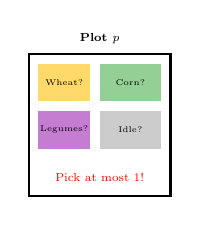
\begin{tikzpicture}[scale=0.6, transform shape]
% Single plot decision
\draw[thick] (0,0) rectangle (3,3);
\node[font=\scriptsize\bfseries, above] at (1.5,3.1) {Plot $p$};

% Options
\fill[cropgold!60] (0.2,2) rectangle (1.3,2.8);
\node[font=\tiny] at (0.75,2.4) {Wheat?};
\fill[cropgreen!60] (1.5,2) rectangle (2.8,2.8);
\node[font=\tiny] at (2.15,2.4) {Corn?};
\fill[croppurple!60] (0.2,1) rectangle (1.3,1.8);
\node[font=\tiny] at (0.75,1.4) {Legumes?};
\fill[gray!40] (1.5,1) rectangle (2.8,1.8);
\node[font=\tiny] at (2.15,1.4) {Idle?};

% Constraint
\node[font=\scriptsize, text=red] at (1.5,0.4) {Pick at most 1!};
\end{tikzpicture}
\end{column}
\end{columns}

\vspace{0.3cm}
\textbf{Interpretation:} $Y_{p,c} = 1$ means ``plant crop $c$ on plot $p$''

\end{frame}

\begin{frame}{Both Approaches Support All Enhancements}

\begin{center}
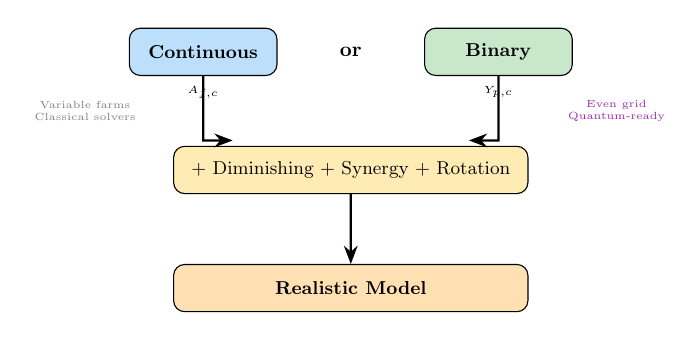
\begin{tikzpicture}[scale=0.75, transform shape,
    block/.style={rectangle, rounded corners, draw, minimum width=2.5cm, minimum height=0.8cm, text centered, font=\small},
    arrow/.style={-Stealth, thick}
]
% Two base models
\node[block, fill=cropblue!30] (cont) at (-2.5,4) {\textbf{Continuous}};
\node[font=\tiny, below=0.05cm of cont] {$A_{f,c}$};
\node[block, fill=cropgreen!30] (bin) at (2.5,4) {\textbf{Binary}};
\node[font=\tiny, below=0.05cm of bin] {$Y_{p,c}$};

% OR label
\node[font=\bfseries] at (0,4) {or};

% Shared enhancements
\node[block, fill=cropgold!30, minimum width=6cm] (enh) at (0,2) {+ Diminishing + Synergy + Rotation};

% Same output
\node[block, fill=croporange!30, minimum width=6cm] (out) at (0,0) {\textbf{Realistic Model}};

% Arrows
\draw[arrow] (cont) -- (-2.5,2.5) -- (-2,2.5);
\draw[arrow] (bin) -- (2.5,2.5) -- (2,2.5);
\draw[arrow] (enh) -- (out);

% Side notes
\node[font=\tiny, text=gray, align=center] at (-4.5,3) {Variable farms\\Classical solvers};
\node[font=\tiny, text=croppurple, align=center] at (4.5,3) {Even grid\\Quantum-ready};
\end{tikzpicture}
\end{center}

\vspace{0.3cm}
\textbf{Key insight:} The formulation choice is about \textit{how we represent land}, not about \textit{what phenomena we model}

\end{frame}

\begin{frame}{Enhancement Options}

\begin{block}{Modular Approach}
Each enhancement can be \textbf{added independently} to capture different real-world phenomena
\end{block}

\vspace{0.3cm}

\begin{enumerate}
    \item \textcolor{cropgreen}{\textbf{Diminishing Returns}} -- Realistic yield curves
    \item \textcolor{cropgold}{\textbf{Crop Synergy}} -- Companion planting benefits  
    \item \textcolor{croppurple}{\textbf{Crop Rotation}} -- Multi-year planning
\end{enumerate}

\vspace{0.5cm}
\textbf{You choose} which features matter for your scenario!

\end{frame}

\begin{frame}{Enhancement 1: Diminishing Returns}

\begin{columns}
\begin{column}{0.5\textwidth}
\textbf{Real-world insight:}\\
Planting 100 ha of wheat doesn't give 10$\times$ the benefit of 10 ha
\begin{itemize}
    \item Market saturation
    \item Pest/disease concentration
    \item Soil depletion
    \item Labor bottlenecks
\end{itemize}

\vspace{0.3cm}
\textbf{Mathematical model:}
\begin{equation*}
\text{Value} = B_c \times A^{0.55}
\end{equation*}

\end{column}

\begin{column}{0.5\textwidth}
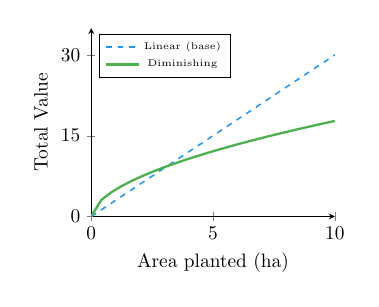
\begin{tikzpicture}[scale=0.7, transform shape]
\begin{axis}[
    xlabel={Area planted (ha)},
    ylabel={Total Value},
    xmin=0, xmax=10,
    ymin=0, ymax=35,
    width=6cm, height=5cm,
    axis lines=left,
    xtick={0,5,10},
    ytick={0,15,30},
    legend pos=north west,
    legend style={font=\tiny}
]
\addplot[cropblue, thick, dashed, domain=0:10] {3*x};
\addlegendentry{Linear (base)}
\addplot[cropgreen, very thick, domain=0:10] {5*x^0.55};
\addlegendentry{Diminishing}
\end{axis}
\end{tikzpicture}

\vspace{0.2cm}
\centering
\scriptsize \textit{Each additional hectare adds less value after a certain point}
\end{column}
\end{columns}

\end{frame}

\begin{frame}{Diminishing Returns: Visual Intuition}

\begin{center}
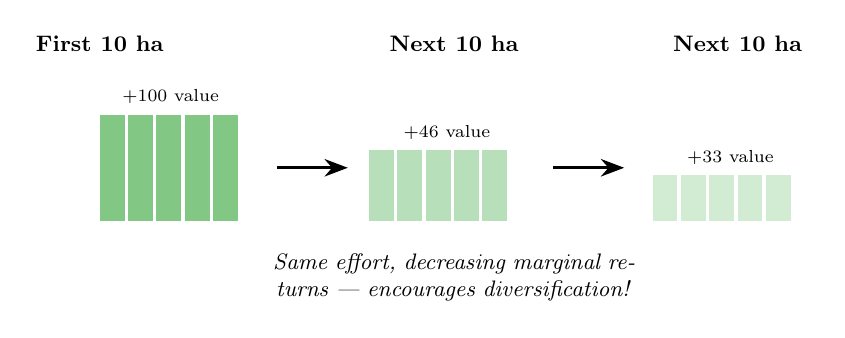
\begin{tikzpicture}[scale=0.9, transform shape]
% First 10 ha
\node[font=\small\bfseries] at (0,2.5) {First 10 ha};
\foreach \i in {0,0.4,0.8,1.2,1.6} {
    \fill[cropgreen!70] (\i,0) rectangle (\i+0.35,1.5);
}
\node at (1,1.75) {\scriptsize +100 value};

% Arrow
\draw[-Stealth, very thick] (2.5,0.75) -- (3.5,0.75);

% Second 10 ha
\node[font=\small\bfseries] at (5,2.5) {Next 10 ha};
\foreach \i in {3.8,4.2,4.6,5,5.4} {
    \fill[cropgreen!40] (\i,0) rectangle (\i+0.35,1);
}
\node at (4.9,1.25) {\scriptsize +46 value};

% Arrow
\draw[-Stealth, very thick] (6.4,0.75) -- (7.4,0.75);

% Third 10 ha
\node[font=\small\bfseries] at (9,2.5) {Next 10 ha};
\foreach \i in {7.8,8.2,8.6,9,9.4} {
    \fill[cropgreen!25] (\i,0) rectangle (\i+0.35,0.65);
}
\node at (8.9,0.9) {\scriptsize +33 value};

% Bottom message
\node[font=\small, text width=10cm, align=center] at (5,-0.8) 
    {\textit{Same effort, decreasing marginal returns --- encourages diversification!}};
\end{tikzpicture}
\end{center}

\end{frame}

\begin{frame}{Diminishing Returns: Performance Impact}

\begin{figure}
    \centering
    \includegraphics[width=\linewidth]{Plots/nln_speedup_comparison.png}
\end{figure}

\scriptsize \textit{Adding this feature increases computation time but captures realistic agricultural economics}

\end{frame}

\begin{frame}{Enhancement 2: Crop Synergy (Companion Planting)}

\begin{columns}
\begin{column}{0.55\textwidth}
\textbf{Real-world insight:}\\
Some crops \textbf{benefit} from being planted together on the same farm:
\begin{itemize}
    \item Nitrogen fixation (legumes help grains)
    \item Pest deterrence
    \item Pollinator attraction
    \item Soil microbiome diversity
\end{itemize}

\vspace{0.3cm}
\textbf{Mathematical model:}
\begin{equation*}
\text{Bonus} = s_{c_1,c_2} \times Y_{c_1} \times Y_{c_2}
\end{equation*}
\end{column}

\begin{column}{0.45\textwidth}
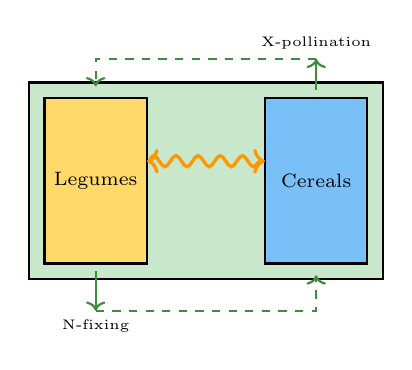
\begin{tikzpicture}[scale=1, transform shape]
% Farm plot with two crops
\draw[thick, fill=cropgreen!30] (0,0) rectangle (4.5,2.5);
% Crop 1 area
\draw[thick, fill=cropgold!60] (0.2,0.2) rectangle (1.5,2.3);
\node[font=\scriptsize] at (0.85,1.25) {Legumes};
% Crop 2 area
\draw[thick, fill=cropblue!60] (3.0,0.2) rectangle (4.3,2.3);
\node[font=\scriptsize] at (3.65,1.25) {Cereals};
% Synergy arrow
\draw[<->, very thick, croporange, decorate, decoration={snake, amplitude=2pt, segment length=8pt}] 
    (1.5,1.5) -- (3.0,1.5);
% % Synergy bonus indicator
% \node[fill=synergyglow, rounded corners, font=\scriptsize\bfseries] at (1.6,2.8) {+Synergy!};
% N-fixation illustration
\draw[->, thick, cropgreen!80!black] (0.85,0.1) -- (0.85,-0.4);
\node[font=\tiny] at (0.85,-0.6) {N-fixing};
% X-pollination illustration
\draw[->, thick, cropgreen!80!black] (3.65,2.4) -- (3.65,2.8);
\node[font=\tiny] at (3.65,3.0) {X-pollination};
% Benefit arrow to cereal (bottom loop)
\draw[->, thick, cropgreen!80!black, dashed] (0.85,-0.4) -- (3.65,-0.4) -- (3.65,0.05);
% Mirrored arrow to complete the loop (top)
\draw[->, thick, cropgreen!80!black, dashed] (3.65,2.8) -- (0.85,2.8) -- (0.85,2.45);
\end{tikzpicture}
\end{column}
\end{columns}

\end{frame}

% \begin{frame}{Synergy: How It Works}

% \begin{center}
% \begin{tikzpicture}[scale=1, transform shape]
% % Synergy matrix visualization
% \node[font=\bfseries] at (2.5,4) {Synergy Matrix};

% % Column headers
% \node[font=\scriptsize] at (1,3.3) {Cereals};
% \node[font=\scriptsize] at (2,3.3) {Legumes};
% \node[font=\scriptsize] at (3,3.3) {Veg};
% \node[font=\scriptsize] at (4,3.3) {Fruits};

% % Row headers  
% \node[font=\scriptsize, right] at (-0.3,2.5) {Cereals};
% \node[font=\scriptsize, right] at (-0.3,1.5) {Legumes};
% \node[font=\scriptsize, right] at (-0.3,0.5) {Veg};

% % Matrix cells
% \fill[gray!30] (0.5,2) rectangle (1.5,3);
% \fill[benefitgreen] (1.5,2) rectangle (2.5,3);
% \fill[gray!20] (2.5,2) rectangle (3.5,3);
% \fill[gray!20] (3.5,2) rectangle (4.5,3);

% \fill[benefitgreen] (0.5,1) rectangle (1.5,2);
% \fill[gray!30] (1.5,1) rectangle (2.5,2);
% \fill[benefitgreen!50] (2.5,1) rectangle (3.5,2);
% \fill[gray!20] (3.5,1) rectangle (4.5,2);

% \fill[gray!20] (0.5,0) rectangle (1.5,1);
% \fill[benefitgreen!50] (1.5,0) rectangle (2.5,1);
% \fill[gray!30] (2.5,0) rectangle (3.5,1);
% \fill[gray!20] (3.5,0) rectangle (4.5,1);

% % Grid lines
% \draw[gray] (0.5,0) grid[step=1] (4.5,3);

% % Values in cells
% \node[font=\tiny] at (1,2.5) {--};
% \node[font=\tiny] at (2,2.5) {\textbf{+0.3}};
% \node[font=\tiny] at (3,2.5) {0};
% \node[font=\tiny] at (4,2.5) {0};

% \node[font=\tiny] at (1,1.5) {\textbf{+0.3}};
% \node[font=\tiny] at (2,1.5) {--};
% \node[font=\tiny] at (3,1.5) {+0.1};
% \node[font=\tiny] at (4,1.5) {0};

% \node[font=\tiny] at (1,0.5) {0};
% \node[font=\tiny] at (2,0.5) {+0.1};
% \node[font=\tiny] at (3,0.5) {--};
% \node[font=\tiny] at (4,0.5) {0};

% % Legend
% \fill[benefitgreen] (5.5,2.5) rectangle (6,3);
% \node[font=\scriptsize, right] at (6,2.75) {Strong synergy};
% \fill[benefitgreen!50] (5.5,1.8) rectangle (6,2.3);
% \node[font=\scriptsize, right] at (6,2.05) {Mild synergy};
% \fill[gray!30] (5.5,1.1) rectangle (6,1.6);
% \node[font=\scriptsize, right] at (6,1.35) {Same crop};
% \end{tikzpicture}
% \end{center}

% \vspace{0.2cm}
% \textbf{Key insight:} The model rewards planting complementary crops together

% \end{frame}

% \begin{frame}{Synergy: Problem Classification}

% \textbf{For Linearized (MILP):}
% \begin{itemize}
%     \item \textbf{Variables:} $2n + |\mathcal{F}| \cdot |\mathcal{S}| \approx 2.3n$
%     \item \textbf{Linearization Constraints:} $3|\mathcal{F}| \cdot |\mathcal{S}|$
% \end{itemize}

% \textbf{For Native Quadratic (MIQP):}
% \begin{itemize}
%     \item \textbf{Variables:} $2n$ (no Z variables needed)
%     \item \textbf{Quadratic Terms:} $O(|\mathcal{F}| \cdot |\mathcal{S}|)$
% \end{itemize}

% \vspace{0.5cm}

% \textbf{Solve Time:} Comparable to linear (1.0-1.5$\times$)

% \end{frame}

\begin{frame}{Synergy: Performance Impact}

\begin{figure}
    \centering
    \includegraphics[width=\linewidth]{Plots/lq_speedup_comparison.png}
\end{figure}


\end{frame}

\begin{frame}{Enhancement 3: Crop Rotation (Multi-Year Planning)}

\textbf{Real-world insight:}\\
What you planted \textbf{last year} affects \textbf{this year's} yield:
\begin{itemize}
    \item Nitrogen replenishment (legumes $\to$ cereals)
    \item Disease cycle breaking
    \item Soil structure restoration
    \item Weed suppression
\end{itemize}

\vspace{0.3cm}
\textbf{Key question:} How do we reward good crop sequences?

\vspace{0.3cm}
\begin{center}
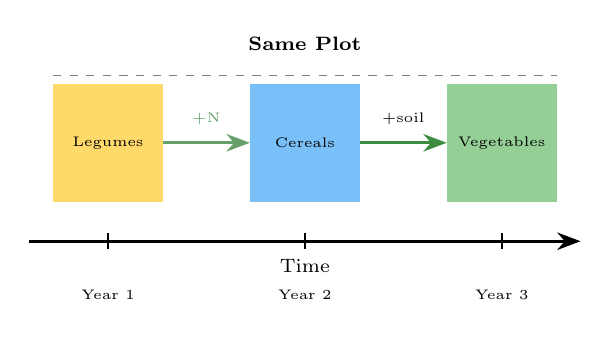
\begin{tikzpicture}[scale=1, transform shape]
% Timeline
\draw[very thick, -Stealth] (0,0) -- (7,0);
\node[below] at (3.5,-0.1) {\scriptsize Time};

% Year markers
\foreach \x/\yr in {1/Year 1, 3.5/Year 2, 6/Year 3} {
    \draw[thick] (\x,0.1) -- (\x,-0.1);
    \node[below] at (\x,-0.5) {\tiny \yr};
}

% Plot visualization
\fill[cropgold!60] (0.3,0.5) rectangle (1.7,2);
\node[font=\tiny] at (1,1.25) {Legumes};

\fill[cropblue!60] (2.8,0.5) rectangle (4.2,2);
\node[font=\tiny] at (3.5,1.25) {Cereals};

\fill[cropgreen!60] (5.3,0.5) rectangle (6.7,2);
\node[font=\tiny] at (6,1.25) {Vegetables};

% Transition arrows with benefits
\draw[-Stealth, very thick, benefitgreen!80!black] (1.7,1.25) -- (2.8,1.25);
\node[above, font=\tiny, text=benefitgreen!80!black] at (2.25,1.35) {+N};

\draw[-Stealth, very thick, cropgreen!80!black] (4.2,1.25) -- (5.3,1.25);
\node[above, font=\tiny] at (4.75,1.35) {+soil};

% Same plot indicator
\node[font=\scriptsize\bfseries, above] at (3.5,2.3) {Same Plot};
\draw[dashed, gray] (0.3,2.1) -- (6.7,2.1);
\end{tikzpicture}
\end{center}

\end{frame}

\begin{frame}{Rotation: The Transition Matrix}

\begin{center}
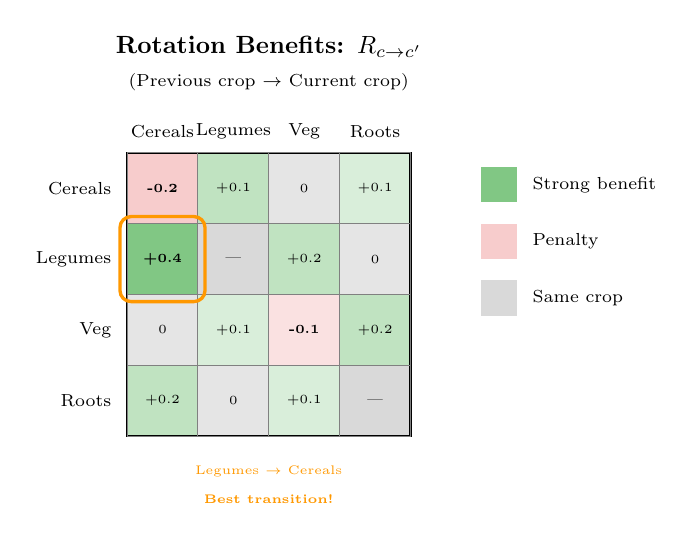
\begin{tikzpicture}[scale=0.9, transform shape]
% Matrix title
\node[font=\bfseries] at (2.5,4.5) {Rotation Benefits: $R_{c \to c'}$};
\node[font=\scriptsize] at (2.5,4.0) {(Previous crop $\to$ Current crop)};

% Column headers (current crop)
\node[font=\scriptsize] at (1,3.3) {Cereals};
\node[font=\scriptsize] at (2,3.3) {Legumes};
\node[font=\scriptsize] at (3,3.3) {Veg};
\node[font=\scriptsize] at (4,3.3) {Roots};

% Row headers (previous crop)
\node[font=\scriptsize, anchor=east] at (0.4,2.5) {Cereals};
\node[font=\scriptsize, anchor=east] at (0.4,1.5) {Legumes};
\node[font=\scriptsize, anchor=east] at (0.4,0.5) {Veg};
\node[font=\scriptsize, anchor=east] at (0.4,-0.5) {Roots};

% Matrix cells with colors
% Row 1: After Cereals
\fill[penaltyred!50] (0.5,2) rectangle (1.5,3);
\fill[benefitgreen!50] (1.5,2) rectangle (2.5,3);
\fill[gray!20] (2.5,2) rectangle (3.5,3);
\fill[benefitgreen!30] (3.5,2) rectangle (4.5,3);

% Row 2: After Legumes
\fill[benefitgreen] (0.5,1) rectangle (1.5,2);
\fill[gray!30] (1.5,1) rectangle (2.5,2);
\fill[benefitgreen!50] (2.5,1) rectangle (3.5,2);
\fill[gray!20] (3.5,1) rectangle (4.5,2);

% Row 3: After Veg
\fill[gray!20] (0.5,0) rectangle (1.5,1);
\fill[benefitgreen!30] (1.5,0) rectangle (2.5,1);
\fill[penaltyred!30] (2.5,0) rectangle (3.5,1);
\fill[benefitgreen!50] (3.5,0) rectangle (4.5,1);

% Row 4: After Roots
\fill[benefitgreen!50] (0.5,-1) rectangle (1.5,0);
\fill[gray!20] (1.5,-1) rectangle (2.5,0);
\fill[benefitgreen!30] (2.5,-1) rectangle (3.5,0);
\fill[gray!30] (3.5,-1) rectangle (4.5,0);

% Grid (draw after fills)
\draw[thick] (0.5,-1) rectangle (4.5,3);
\draw[gray] (0.5,-1) -- (0.5,3);
\draw[gray] (1.5,-1) -- (1.5,3);
\draw[gray] (2.5,-1) -- (2.5,3);
\draw[gray] (3.5,-1) -- (3.5,3);
\draw[gray] (4.5,-1) -- (4.5,3);
\draw[gray] (0.5,-1) -- (4.5,-1);
\draw[gray] (0.5,0) -- (4.5,0);
\draw[gray] (0.5,1) -- (4.5,1);
\draw[gray] (0.5,2) -- (4.5,2);
\draw[gray] (0.5,3) -- (4.5,3);

% Values
\node[font=\tiny] at (1,2.5) {\textbf{-0.2}};
\node[font=\tiny] at (2,2.5) {+0.1};
\node[font=\tiny] at (3,2.5) {0};
\node[font=\tiny] at (4,2.5) {+0.1};

\node[font=\tiny] at (1,1.5) {\textbf{+0.4}};
\node[font=\tiny] at (2,1.5) {---};
\node[font=\tiny] at (3,1.5) {+0.2};
\node[font=\tiny] at (4,1.5) {0};

\node[font=\tiny] at (1,0.5) {0};
\node[font=\tiny] at (2,0.5) {+0.1};
\node[font=\tiny] at (3,0.5) {\textbf{-0.1}};
\node[font=\tiny] at (4,0.5) {+0.2};

\node[font=\tiny] at (1,-0.5) {+0.2};
\node[font=\tiny] at (2,-0.5) {0};
\node[font=\tiny] at (3,-0.5) {+0.1};
\node[font=\tiny] at (4,-0.5) {---};

% Legend
\fill[benefitgreen] (5.5,2.3) rectangle (6,2.8);
\node[font=\scriptsize, anchor=west] at (6.1,2.55) {Strong benefit};
\fill[penaltyred!50] (5.5,1.5) rectangle (6,2.0);
\node[font=\scriptsize, anchor=west] at (6.1,1.75) {Penalty};
\fill[gray!30] (5.5,0.7) rectangle (6,1.2);
\node[font=\scriptsize, anchor=west] at (6.1,0.95) {Same crop};

% Highlight example
\draw[very thick, croporange, rounded corners] (0.4,0.9) rectangle (1.6,2.1);
\node[font=\tiny, croporange, below] at (2.5,-1.3) {Legumes $\to$ Cereals};
\node[font=\tiny, croporange, below] at (2.5,-1.7) {\textbf{Best transition!}};
\end{tikzpicture}
\end{center}

\end{frame}

\begin{frame}{Rotation: Mathematical Formulation}

\textbf{Extended objective over multiple periods:}
\begin{equation*}
\max \underbrace{\sum_{t=1}^{T} \sum_{f,c} B_c \cdot A_{f,c,t}}_{\text{crop values per period}}
+ \gamma \underbrace{\sum_{t=2}^{T} \sum_{f,c,c'} R_{c,c'} \cdot Y_{f,c,t-1} \cdot Y_{f,c',t}}_{\text{rotation rewards}}
\end{equation*}

\vspace{0.3cm}

\begin{columns}
\begin{column}{0.5\textwidth}
\textbf{New elements:}
\begin{itemize}
    \item $t$: Time period (year/season)
    \item $R_{c,c'}$: Transition benefit matrix
    \item $\gamma$: Rotation importance weight
\end{itemize}
\end{column}

\begin{column}{0.5\textwidth}
\textbf{What this captures:}
\begin{itemize}
    \item Multi-year planning horizon
    \item Sequential crop interactions
    \item Long-term soil health
\end{itemize}
\end{column}
\end{columns}

\vspace{0.4cm}
\textbf{You provide:} The $R_{c,c'}$ matrix based on agronomic knowledge!

\end{frame}

\begin{frame}{Putting It All Together}

\begin{center}
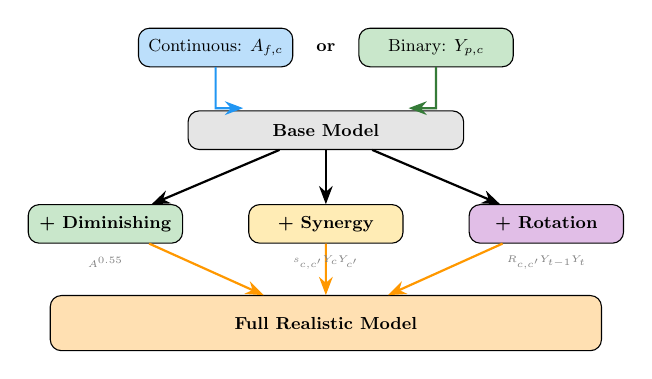
\begin{tikzpicture}[scale=0.7, transform shape,
    box/.style={rectangle, rounded corners, draw, minimum width=2.8cm, minimum height=0.7cm, text centered, font=\small}
]
% Two base models at top
\node[box, fill=cropblue!30] (cont) at (-2,5) {Continuous: $A_{f,c}$};
\node[box, fill=cropgreen!30] (bin) at (2,5) {Binary: $Y_{p,c}$};
\node[font=\small\bfseries] at (0,5) {or};

% Combined base
\node[box, fill=gray!20, minimum width=5cm] (base) at (0,3.5) {\textbf{Base Model}};

% Enhancements
\node[box, fill=cropgreen!30] (dim) at (-4,1.8) {\textbf{+ Diminishing}};
\node[box, fill=cropgold!30] (syn) at (0,1.8) {\textbf{+ Synergy}};
\node[box, fill=croppurple!30] (rot) at (4,1.8) {\textbf{+ Rotation}};

% Full model
\node[box, fill=croporange!30, minimum width=10cm, minimum height=1cm] (full) at (0,0) {
    \textbf{Full Realistic Model}
};

% Arrows from bases
\draw[-Stealth, thick, cropblue] (cont) -- (-2,3.9) -- (-1.5,3.9);
\draw[-Stealth, thick, cropgreen!70!black] (bin) -- (2,3.9) -- (1.5,3.9);

% Arrows to enhancements
\draw[-Stealth, thick] (base) -- (dim);
\draw[-Stealth, thick] (base) -- (syn);
\draw[-Stealth, thick] (base) -- (rot);

% Arrows to full model
\draw[-Stealth, thick, croporange] (dim) -- (full);
\draw[-Stealth, thick, croporange] (syn) -- (full);
\draw[-Stealth, thick, croporange] (rot) -- (full);

% Annotations
\node[font=\tiny, text=gray] at (-4,1.1) {$A^{0.55}$};
\node[font=\tiny, text=gray] at (0,1.1) {$s_{c,c'} Y_c Y_{c'}$};
\node[font=\tiny, text=gray] at (4,1.1) {$R_{c,c'} Y_{t-1} Y_t$};
\end{tikzpicture}
\end{center}

\vspace{0.2cm}
\textbf{Your input needed:}
\begin{itemize}
    \item Synergy matrix $s_{c,c'}$: Which crops benefit from co-location?
    \item Rotation matrix $R_{c,c'}$: Which sequences are agronomically beneficial?
\end{itemize}

\end{frame}



\begin{frame}{Summary: A Modular Toolkit}

\begin{table}
\centering
\small
\begin{tabular}{@{}lll@{}}
\toprule
\textbf{Enhancement} & \textbf{Captures} & \textbf{You Provide} \\
\midrule
Diminishing Returns & Market saturation & Exponent $\alpha$ \\
                    & Resource limits   & (we suggest 0.55) \\
\midrule
Crop Synergy        & Companion planting & Matrix $s_{c,c'}$ \\
                    & Ecosystem services & \\
\midrule
Crop Rotation       & Multi-year planning & Matrix $R_{c,c'}$ \\
                    & Soil health         & Weight $\gamma$ \\
\bottomrule
\end{tabular}
\end{table}

\vspace{0.5cm}
\textbf{Key message:} The model is \textbf{flexible} --- we add complexity where it helps capture your agricultural reality

\end{frame}

\begin{frame}{Benchmark: Results}

\begin{figure}
    %\centering
    \adjincludegraphics[width=0.9\linewidth , trim={0 {0.5\height} 0 0},clip]{Plots/largest_config_combined.pdf}
\end{figure}

\end{frame}


\begin{frame}{Benchmark: Results}

\begin{figure}
    %\centering
    \adjincludegraphics[width=0.9\linewidth , trim={0 0 0 {0.5\height}},clip]{Plots/largest_config_combined.pdf}
\end{figure}

\end{frame}

\begin{frame}{Tuning the Model: Crop Benefit Importances}

\textbf{How do we calculate the ``value'' of each crop?}

\vspace{0.3cm}

The benefit score $B_c$ for each crop combines multiple factors:

\vspace{0.3cm}

\begin{columns}
\begin{column}{0.5\textwidth}
\textbf{Current Importances:}
\begin{itemize}
    \item Nutritional Value: \textbf{20\%}
    \item Nutrient Density: \textbf{20\%}
    \item Affordability: \textbf{20\%}
    \item Sustainability: \textbf{20\%}
    \item Environmental Impact: \textbf{20\%}
\end{itemize}
\end{column}

\begin{column}{0.5\textwidth}
\textbf{Questions for you:}
\begin{itemize}
    \item Is nutrition more important than affordability?
    \item Should sustainability weigh more heavily?
    \item Are there other factors to include?
\end{itemize}
\end{column}
\end{columns}

\vspace{0.5cm}

\begin{block}{Your Input}
These importances are fully adjustable. Tell us what matters most for your application, and we'll update the model accordingly!
\end{block}

\end{frame}

\end{document}
